\documentclass{article}
\usepackage{listings}
\usepackage{amsmath}
\usepackage{amssymb}
\usepackage[linesnumbered, boxruled]{algorithm2e}
\usepackage{graphicx}
\graphicspath{ {/home/saurabh/studies/Spring2016/algorithms/assignment-5/} }
\providecommand{\e}[1]{\ensuremath{\times 10^{#1}}}
\bibliographystyle{plain}
\usepackage{url}
\begin{document}

\begin{center}{\LARGE Fast Fourier Transform}\end{center}
\begin{center}{\normalsize Saurabh Sood}\end{center}

\begin{abstract}
This paper presents the implementation and analysis of the Fast Fourier Transform. The Fast Fourier transform algorithm is a major asymptotic improvement over the Discrete Fourier transform, and has varied applications in the field of signal processing. The Discrete Fourier Transform (DFT) has a time complexity of $O(n^2)$, whereas the Fast Fourier Transform runs in $O(nlog_2{n})$. The paper looks at an implementation of the FFT, and provides a rigorous mathematical analysis of the time, and space complexities in the Worst, Average and Best case inputs. 
\end{abstract}

\section{Introduction}
The Discrete Fourier Transform (DFT) is the most important transformation used in Fourier Analysis. It is used to convert a set of function values into a combination of periodic functions (namely sine waves). More intuitively, it can be thought of as converting a function from the time domain to the frequency domain. This has various applications in the field of Image Processing, Digital Signal Processing to name a few. In the field of Digital Signal Processing, it can be used to find the various frequencies in a noisy channel, whereas in Image Processing, it can be used to extract the actual image from a blurred image, by clearing out the noisy pixels. In Mathematics, it can be used to solve Partial Differential Equations really fast.  It is such an important algorithm, that special hardware is built so that it runs really fast. In hardware, the DFT is usually implemented with the Fast Fourier Transform (FFT) algorithm, which is an asymptotically faster algorithm for the DFT.

\section{History}
The DFT can be traced to the work done by Fourier, who proposed that a function could be represented as a combination of sinusoidal functions. However, the algorithm to compute the DFT was inefficient, and could not run on most hardware at that time. There was work done by Gauss for a fast running implementation of the DFT, but it was never published \cite{10.2307/2003354}. Currently, the most commonly used version of the FFT can be traced to the work done by Cooley, an IBM engineer, and Tukey, a statistician. Their work involved improving the algorithm, so that it works when their input size is not a power of 2 as well.

\section{The Discrete Fourier Transform}
%The DFT is used to represent a set of points in a function as a combination of sinusoidal functions. Intuitively, this could be imagined as representing the set of points in the frequency domain. The points in function could represent different things based on the application. For example, in the case of Digital Signal Processing, the signal could be represented as a function of time. \\
%
%The input to the DFT is a sample of complex numbers, and the output is a set of complex coefficients formed from a combination of sinusoidal waves. Mathematically, the DFT can be represented as follows: \\ \\
%$\sum_{n=0}^{N-1}x_{n}e^{\frac{-2\pi ikn}{N}}$, for $k \in \mathbb{Z}$ \\ \\
%where $x_{0}, x_{1}...x_{N-1}$ represent the input sequence of numbers, which are part of the function being transformed \\
%$e^{\frac{-2\pi ikn}{N}}$ represents the complex sinusoidal waveforms used to transform the given input.
\subsection{Complex Roots of Unity}
A complex $n^th$ root of unity is a complex number $\omega$ such that \\
\begin{center}
$\omega^{n}=1$ \\
\end{center}
The $n$ complex roots of unity can be represented as follows:
\begin{center}
$e^{\frac{2\pi ik}{n}}$; for $k=0,1,2...n-1$
\end{center}
This can be represented trigonometrically as:
\begin{center}
$e^{iu}=cos(u)+isin(u)$
\end{center}
Pictorially, the roots of unity can be represented as shown in the following figure: \\
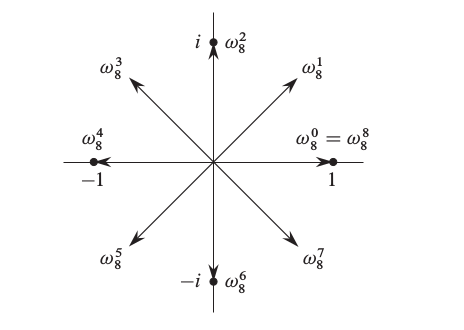
\includegraphics[scale=0.5]{roots} \\
where the values of $w_{8}^{0}...w_{8}^{7}$ are represented in the complex plane, and $w_{8}=e^{\frac{2\pi\i}{8}}$ is the principal $8^{th}$ root of unity

\subsection{Cancellation Lemma}
\begin{center}
$\omega_{dn}^{dk}=\omega_{n}^{k}$; for $n \geq 0, k \geq 0, d>0$ \\
\end{center}
This follows directly from the definition of the complex roots of unity:
\begin{center}
$\omega_{n}=e^{\frac{2\pi i}{n}}$
\end{center} 

\subsection{Halving Lemma}
\begin{center}
$(\omega_{n}^{\frac{k+n}{2}})^{2}=(\omega_{n}^{k})^{2}$; if $n>0$ is even
\end{center}
This implies that for an even value of $n$, the squares of the $n$ complex roots of unity are the $\frac{n}{2}$ complex $(\frac{n}{2})^{th}$ roots of unity

\subsection{Summation Lemma}
\begin{center}
$\sum_{j=0}^{n-1}(\omega_{n}^{k})^{j}=0$; for $n \geq 1$, and for $k$ not divisible by n
\end{center}
The increasing powers of complex roots of unity sum to 0

\subsection{The Algorithm}
The Discrete Fourier transform can be represented with the following conversion: \\
\begin{center}

\begin{align*}
y_{k}&=A(w_{n}^{k}) \\
&=\sum_{j=0}^{n-1}{a_{j}\omega_{n}^{kj}}
\end{align*}
\end{center}
for $k=0,1,2...,n-1$, and $a_{j}$ is the coefficient matrix of a polynomial $A(x)$ \\
\begin{center}
$A(x)=\sum_{j=0}^{n-1}{a_{j}x^{j}}$
\end{center}
The vector $y=(y_{0},y_{1}...y_{n-1}$ is called the \textit{Discrete Fourier Transform} of the coefficient vector $a=(a_{0}, a_{1},...,a_{n-1})$

\subsection{Pseudocode}
\begin{algorithm}[H]
 \KwData{An input coefficient vector $a$}
 \KwResult{A vector $y$, of length $n$, which is the Discrete Fourier Transform of the given input coefficient vector $a$}
 initialization\;
 $n=a.length$ ;where n is a power of 2  \\
 \eIf{n==1} {
 	\textbf{return a}
 }{
 	\For{$k=0\ to\ n$}{
 		$sum=0$ \\
 		\For{$j=0\ to\ n-1$}{
 			$sum += a_{j}e^{\frac{-2\pi ijk}{n}}$
 		}
 		$y_{k}=sum$
 	}
 	\textbf{return y}
 }
 \caption{$O(n^{2})$ implementation of the Discrete Fourier Transform}
\end{algorithm}

\subsection{Analysis of the DFT}
\textbf{Time Complexity} \\
The above algorithm for computing the Discrete Fourier Transform has a time complexity of $O(n^{2})$. 
\begin{itemize}
\item The inner loop computes the $k_{th}$ coefficient of the output vector. Mathematically, it represents:
\begin{center}
$y_{k}=\sum_{j=0}^{n-1}a_{k}e^{\frac{-2\pi ijk}{n}}$
\end{center}
This takes $n$ iterations
\item
The outer loop computes the coefficient for each of the $n$ input vectors. This also takes $n$ iterations.
\end{itemize}

Thus, the overall time complexity is $O(n^{2})$ \\

\textbf{Runtime Analysis for Best Case, Worst Case, Average Case Inputs}
\begin{itemize}
\item
The best case input for the algorithm will be when the input vector is of size $1$, in which case the algorithm will return the input vector itself. In this case, the algorithm will run in $O(1)$ time.
\item
There is no worst case input for the DFT algorithm. In the average case, the input vector is of size $n$. The DFT in this case would return a vector of size $n$. The runtime complexity of the algorithm in this case would be $O(n^{2})$.
\end{itemize}

\textbf{Numerical Characterization of the Running Time} \\ \\
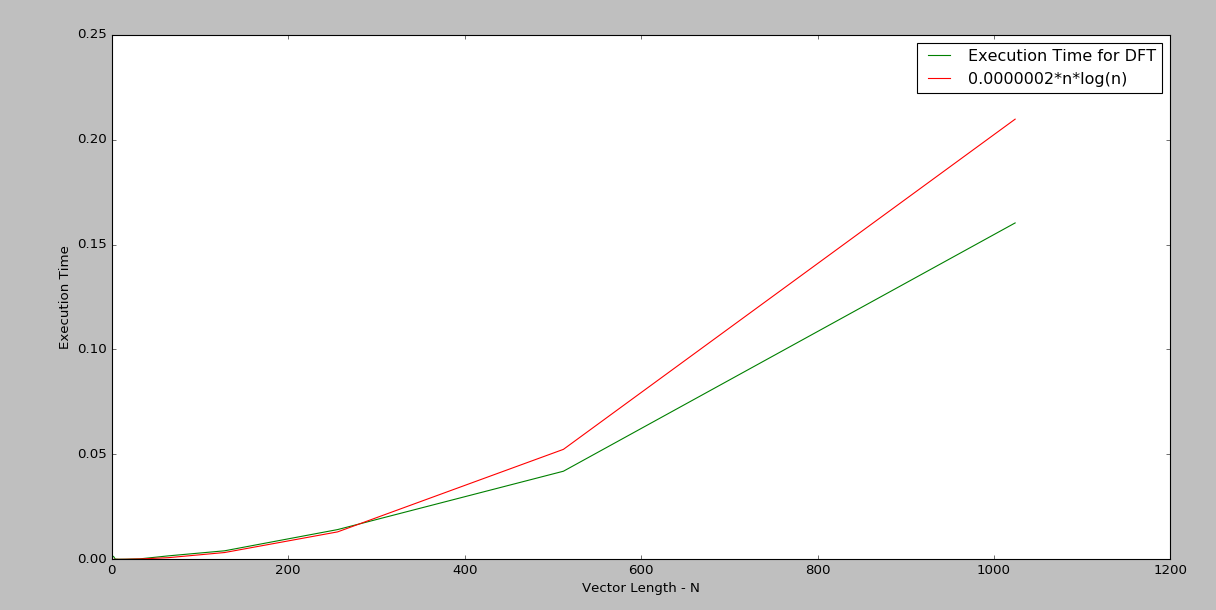
\includegraphics[scale=0.3]{dft}
\begin{center}
Plot showing the runtime of DFT.  \\
\end{center}
The input here is a vector of length 2-1024 (Due to limitations in RAM, it could not be extended for further values of $N$). The y-axis of the graph represents the running time of the algorithm. Here, the input vector $a$ is randomly generated. The graph shows a $O(n^{2})$ bound for the runtime of the algorithm.\\ \\
The graph for the running time for the DFT in semilogx scale is as shown below: \\ \\
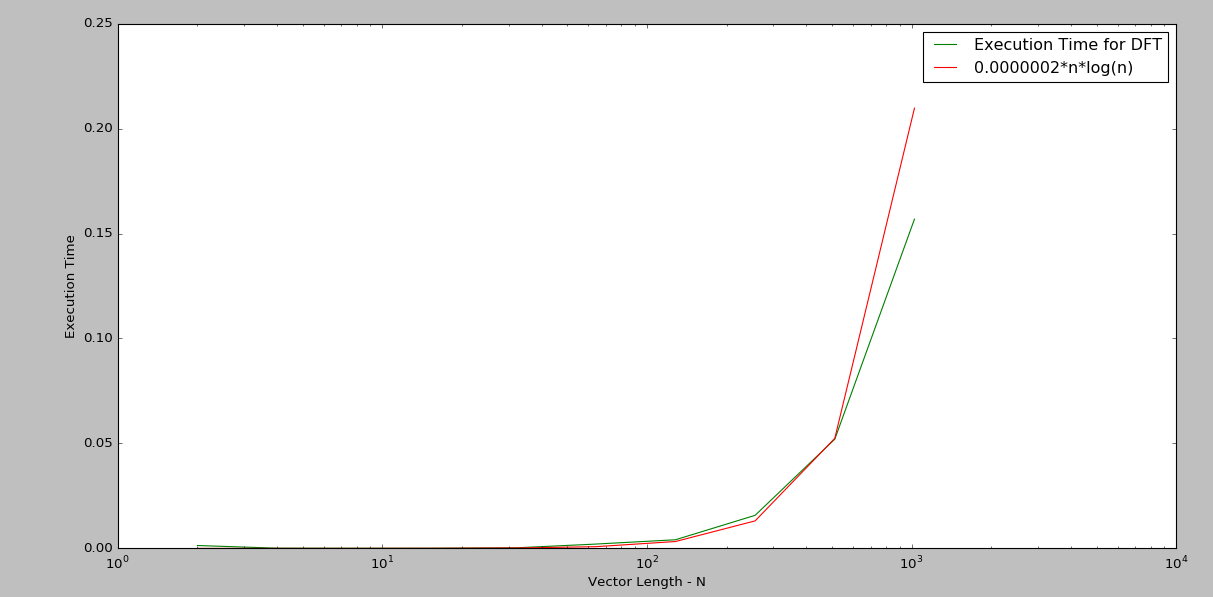
\includegraphics[scale=0.3]{logscale-dft} \\ \\


\textbf{Space Complexity}
\begin{itemize}
\item The input and output vectors are of length $n$ each. Both take $O(n)$ space.
\item The intermediate \textit{sum} variable takes $O(1)$ space
\end{itemize}
Thus, the overall space complexity of the algorithm is $O(n)$


\section{Fast Fourier Transform} \cite{fft}
The Discrete Fourier Transform(FFT) runs in $O(n^{2})$ running time, where $n$ is the polynomial vector length. The algorithm showed earlier doesn't scale well for very high powers of $n$. The Fast Fourier Transform algorithm takes advantage of special properties like symmetry, in the computing the roots, and reduces the computational time taken for computing the Discrete Fourier Transform. The runtime complexity of the FFT is $O(nlog{n})$, as opposed to $O(n^{2})$ in the base version of the DFT. \\

\subsection{The Algorithm}
For the purpose of the paper, we assume that $n$ is a power of 2. The FFT works for non-powers of 2, but the assumption makes the analysis easier. The FFT is a divide and conquer algorithm. It separately considers the even and odd coefficients of $A(x)$ \\

$A^{[0]}(x)=a_{0}+a_{2}x+a_{4}x^{2}+...+a_{n-2}x^{\frac{n}{2}-1}$ \\
$A^{[1]}(x)=a_{1}+a_{3}x+a_{5}x^{2}+...+a_{n-1}x^{\frac{n}{2}-1}$ \\

where $A^{[0]}(x)$ considers the even coefficients of $A(x)$, and $A^{[1]}(x)$ considers the odd coefficients of $A(x)$ \\
The problem of computing the DFT can be summarized with the following: \\
\begin{itemize}
\item
\textbf{Divide Step} \\
evaluating the $\frac{n}{2}$ polynomials $A^{[0]}(x)$ and $A^{[1]}(x)$ at the points $(\omega_{n}^{0})^{2},(\omega_{n}^{1})^{2},...,(\omega_{n}^{n-1})^{2}$
\item
\textbf{Conquer Step} \\
Combine the results using the formula: \\
\begin{center}
$A(x)=A^{[0]}(x^{2})+A^{[1]}(x^{2})$
\end{center}
\end{itemize}
Using the Halving Lemma, the polynomial evaluations at $(\omega_{n}^{0})^{2},(\omega_{n}^{1})^{2},...,(\omega_{n}^{n-1})^{2}$ consist of the $\frac{n}{2}$ complex $\frac{n}{2}^{th}$ roots of unity with each root occuring twice. Thus, we have two subproblems of the same form as the original problem, and are half the size of the original problem. This leads to a recursive algorithm for the FFT, where the original problem of $DFT_{n/2}$ reduces to two problems of $DFT_{n/2}$

\subsection{Analysis} \cite{Cormen:2001:IA:580470}
\begin{algorithm}[H]
 \KwData{An input coefficient vector $a$}
 \KwResult{A vector of length $n$, which is the Discrete Fourier Transform of the given input coefficient vector $a$}
 initialization\;
 $n=a.length$ ;where n is a power of 2  \\
 \eIf{n==1} {
 	\textbf{return a}
 }{
 	$\omega_{n}=e^{\frac{2\pi i}{n}}$ \\
 	$\omega=1$ \\
 	$a^{[0]}=(a^{0},a^{2},...,a^{n-2}$ \\
 	$a^{[1]}=(a^{1},a^{3},...,a^{n-1}$ \\
 	$y^{[0]}=RECURSIVE\_FFT(a^{[0]})$ \\
 	$y^{[1]}=RECURSIVE\_FFT(a^{[1]})$ \\
 	\For{$k=0\ to\ \frac{n}{2}-1$}{
 		$y_{k}=y_{k}^{[0]}+\omega y_{k}^{[1]}$ \\
 		$y_{k+\frac{n}{2}}=y_{k}^{[0]}-\omega y_{k}^{[1]}$ \\
 		$\omega=\omega \omega_{n}$
 	}
 	\textbf{return y}
 }
 \caption{Recursive Implementation of the Fast Fourier Transform}
\end{algorithm}

\begin{itemize}
\item
Lines 3-4 represent the base case of the recursion, where the DFT of a single element is the element itself
\item
Lines 8-9 define the coefficient vectors for the polynomials $A^{[0]}$, and $A^{[1]}$.
\item
Lines 6,7,15 ensures that $\omega$ is updated whenever the DFT coefficient vectors get updated in Lines 13,14. Thus, we will always have
\begin{center}
$\omega=\omega_{n}^{k}$
\end{center}
\item
Lines 10, 11 perform the recursive $DFT_{\frac{n}{2}}$ computations. The for loop runs for $k=0,1,2...\frac{n}{2}-1$ iterations. So, we have:
\begin{center}
$y_{k}^{[0]}=A^{[0]}(\omega_{\frac{n}{2}}^{k})^{2}$ \\
$y_{k}^{[1]}=A^{[1]}(\omega_{\frac{n}{2}}^{k})^{2}$ \\
\end{center}
Since $\omega_{\frac{n}{2}{k}}=\omega_{n}^{2k}$ (Cancellation Lemma), we have the following results: \\
\begin{center}
$y_{k}^{[0]}=A^{[0]}(\omega_{n}^{2k})^{2}$ \\
$y_{k}^{[1]}=A^{[1]}(\omega_{n}^{2k})^{2}$ \\
\end{center}
\item
Lines 13,14 combine the results of the $DFT_{n/2}$ computations. We get the following results:
\begin{center}
\begin{align*}
y_{k}&=y_{k}^{0}+\omega_{n}^{k}y_{k}^{[1]} \\
&=A^{[0]}(\omega_{n}^{2k})+\omega_{n}^{k}A^{[1]}(\omega_{n}^{2k}) \\
&=A(\omega_{n}^{k})
\end{align*}
\end{center}
\item
For $y_{\frac{n}{2}}, y_{\frac{n}{2}-1}...y_{n-1}$, setting $k=0,1,...,\frac{n}{2}-1$ yields: \\
\begin{center}
\begin{align*}
y_{k+\frac{n}{2}}&=y_{k}^{[0]}-\omega_{n}^{k}y_{k}^{[1]} \\
&=y_{k}^{[0]}+\omega_{n}^{k+\frac{n}{2}}y_{k}^{[1]} \text{; since } \omega_{n}^{k+\frac{n}{2}=-\omega_{n}^{k}} \\
&=A^{[0]}(\omega_{n}^{2k})+\omega_{n}^{k+\frac{n}{2}}A^{[1]}(\omega_{n}^{2k}) \text{; since } \omega_{n}^{2k+n}=\omega_{n}^{2k} \\
&=A^{[0]}(\omega_{n}^{2k+n})+\omega_{n}^{k+\frac{n}{2}}A^{[1]}(\omega_{n}^{2k+n}) \\
&=A(\omega_{n}^{k+\frac{n}{2}})
\end{align*}
\end{center}
Thus, we get the same vector which is the same as the output of the DFT of the input vector $a$. 
\end{itemize}

\subsection{Runtime Analysis}
To find the running time of the \textit{RECURSIVE\_FFT} procedure, we note that each invocation (aside from the recursive step) takes $\theta(n)$ time. Thus, we can form the following recurrence: \\
\begin{align*}
T(n)&=2T(\frac{n}{2})+\Theta(n) \\
&=\Theta(nlgn) \text{ ; Using the master theorem}
\end{align*}
Thus, the Fast Fourier Transform is an asymptotic upgrade over the basic implementation of the Discrete Fourier Transform

\subsection{Runtime Analysis for Worst Case, Average Case Inputs}
\textbf{Average Case/Worst Case inputs} \\
There is no worst case input for the FFT algorithm. In the general case, the coefficient vector is a vector of length $n$, where $n=2^{k}$; $k>0$. \\
In this case, the algorithm will take $O(nlogn)$ time.

\subsection{Numerical Characterization of the Runtime}

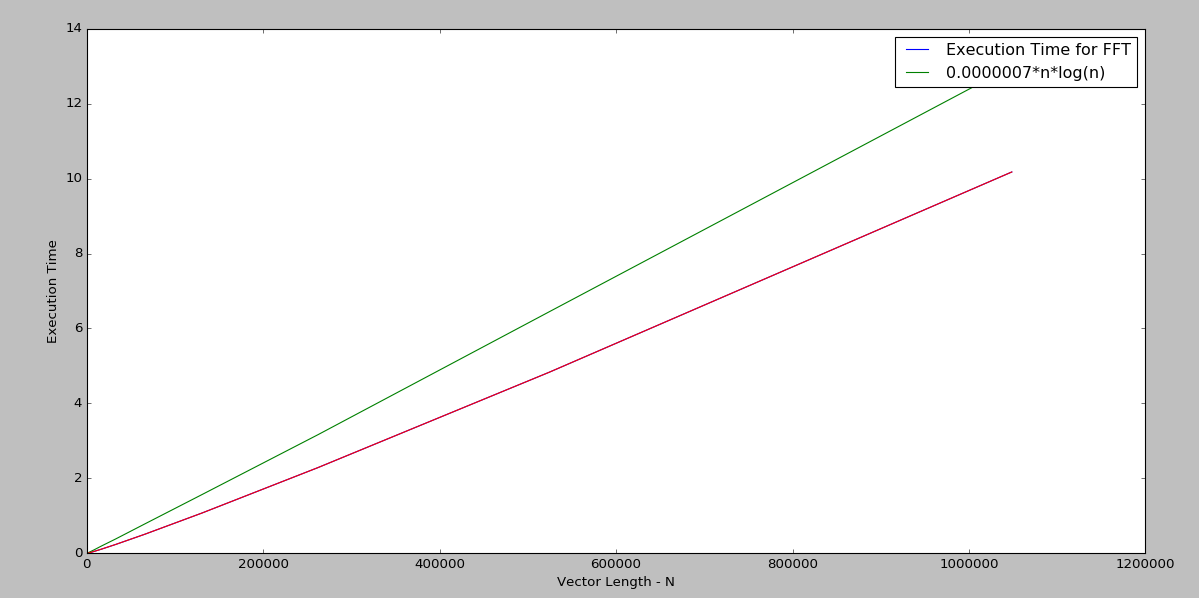
\includegraphics[scale=0.3]{fft}
\begin{center}
Plot showing the runtimes of FFT
\end{center}
The input here is a vector of length 2-1048576 ($2^{0}$ to $2^{20}$). The y-axis of the graph represents the running time of the algorithm. Here, the input vector $a$ is randomly generated. The graph shows a $O(nlog(n))$ bound for the algorithm. \\ \\
The graph for the running time for the FFT in semilogx scale is as shown below: \\ \\
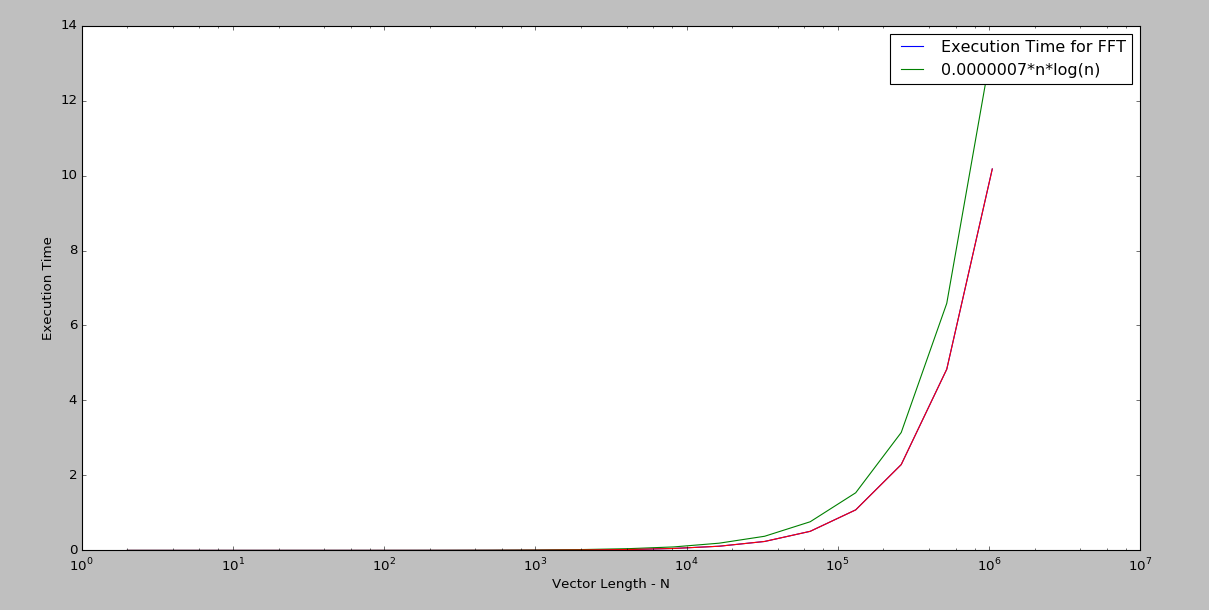
\includegraphics[scale=0.3]{fft-logscale}

\subsection{Space Complexity}
\begin{itemize}
\item
The input and output vectors take $O(n)$ space
\item
The computations and multiplications take $O(1)$ extra space
\end{itemize}

Thus, the overall space complexity of the algorithm is $O(n)$

\subsection{Extensions}
The paper explored the Discrete Fourier Transform, it's runtime, and space complexity. It also explored the improvements done with using the $FFT$ algorithm, and showed that it is an asymptotic improvement over the base DFT algorithm. \\
There are some extensions for the analysis of the DFT and FFT done in the paper, which could be done.
\begin{itemize}
\item
Due to RAM limitations, the base DFT algorithm could be run for only a small set of values ($2^{10}$). The algorithm could be run on a faster computer (or a supercomputer) to clearly show the $O(n^{2})$ bound for a larger set of values.
\item
The algorithms presented in the section run for input vectors having length as a power of 2. This makes the algorithm easier to analyze. However, FFT and DFT run on input vectors of arbitrary sizes. For future work, this could be incorporated in the implementation and the analysis.
\end{itemize}


\bibliography{main}
\end{document}